\section{Fase II: Planeación}

La fase de planeación establece el marco de trabajo con el que el equipo de siete integrantes desarrolla el Sistema Web de Compra de Materiales de Escritorio, orientado al modelo B2C (\textit{Business to Consumer}). En ella se delimita el alcance del proyecto, se estiman los recursos y el esfuerzo, se define el cronograma iterativo conforme al Proceso Unificado Ágil (AUP), se identifican y gestionan los riesgos mediante la estrategia RMMM de Pressman (Reducción, Supervisión y Gestión del Riesgo) y se establecen los mecanismos de seguimiento, el control de configuración y los criterios que determinan cuándo un entregable se considera terminado.

\subsection{Definición del Alcance y Delimitación del Proyecto}
\label{subsec:alcance_delimitacion}

Considerando la naturaleza y el alcance establecidos para el proyecto de asignatura, el trabajo se acota estrictamente hasta la etapa de diseño detallado y especificación técnica, bajo los siguientes límites:

\subsubsection*{Incluido en el alcance (Fases de Comunicación, Planeación y Modelado)}
\begin{itemize}
    \item \textbf{Ingeniería de Requerimientos y Alcance B2C:} Definición formal de actores, 18 requerimientos funcionales (\texttt{RF01}--\texttt{RF18}), 11 requerimientos no funcionales (\texttt{RNF01}--\texttt{RNF11}), glosario técnico y casos de uso generales y expandidos.
    \item \textbf{Modelado Estructural y de Datos:} Diagrama de clases del dominio y del sistema, modelo entidad-relación (E-R), esquema relacional normalizado y diccionario de datos en MySQL.
    \item \textbf{Modelado Dinámico y de Comportamiento:} Diagramas de secuencia, de actividades y de máquina de estados para los flujos críticos (registro, catálogo, carrito, validación de \textit{stock}, confirmación y gestión administrativa de pedidos).
    \item \textbf{Modelado Arquitectónico y Prototipado UX/UI:} Diagramas de componentes y de despliegue (arquitectura cliente-servidor web) y prototipos visuales navegables (\textit{wireframes} y \textit{mockups}) de las interfaces de Cliente y Administrador.
\end{itemize}

\subsubsection*{Excluido del alcance (fases posteriores y limitaciones funcionales)}
\begin{itemize}
    \item \textbf{Construcción y Despliegue (codificación):} No se contempla el desarrollo del código fuente productivo (Backend/Frontend), la puesta en marcha en servidores reales ni las pruebas de estrés en producción; estas actividades quedan proyectadas para una etapa posterior de implementación.
    \item \textbf{Pasarela de pagos electrónicos y rastreo GPS:} Dentro de la lógica modelada, los pedidos se confirman mediante la validación de disponibilidad en inventario y se gestionan por estados administrativos (\textit{Recibido}, \textit{En preparación}, \textit{En camino} y \textit{Entregado}), sin cobros en línea ni geolocalización.
\end{itemize}

Toda solicitud que exceda estos límites se tramita como solicitud de cambio, según el procedimiento de control de configuración establecido por el equipo.

\subsection{Estimación de Recursos}

Para ejecutar el proyecto dentro del calendario académico de la asignatura se asignan los siguientes recursos humanos, de hardware y de software.

\subsubsection{Recursos humanos (equipo de desarrollo: 7 integrantes)}

El equipo adopta una estructura colaborativa propia de AUP y concentra a la totalidad de sus integrantes en las disciplinas de análisis, modelado UML, diseño de datos y prototipado de interfaz. Cada artefacto tiene un responsable único y es revisado por un integrante distinto de su autor, tal como se detalla en la Tabla \ref{tab:roles_equipo}.

{\small
\begin{xltabular}{\textwidth}{|>{\raggedright\arraybackslash}p{2.8cm}|X|>{\raggedright\arraybackslash}p{3.6cm}|>{\raggedright\arraybackslash}p{1.8cm}|}
    % --- Título y encabezado de la PRIMERA página ---
    \caption{Roles, responsabilidades y artefactos del equipo}
    \label{tab:roles_equipo} \\
    \hline
    \textbf{Rol en el proyecto} & \textbf{Responsabilidades} & \textbf{Artefactos asociados} & \textbf{Iteraciones} \\
    \hline
    \endfirsthead

    % --- Encabezado que se repite en las páginas SIGUIENTES ---
    \multicolumn{4}{l}{\textit{Continuación de la Tabla \ref{tab:roles_equipo}}} \\
    \hline
    \textbf{Rol en el proyecto} & \textbf{Responsabilidades} & \textbf{Artefactos asociados} & \textbf{Iteraciones} \\
    \hline
    \endhead

    % --- Pie de tabla en páginas intermedias ---
    \multicolumn{4}{r}{\textit{Continúa en la siguiente página...}} \\
    \endfoot

    % --- Pie final de la tabla (con nota aclaratoria) ---
    \multicolumn{4}{l}{\footnotesize \textit{Nota:} En la Iteración 1 participa todo el equipo; el total de integrantes distribuidos por rol suma 7.} \\
    \endlastfoot

    % --- Contenido de las filas ---
    Líder de proyecto / coordinador & Planificación de iteraciones, seguimiento del cronograma, gestión de riesgos (RMMM), conducción de los \textit{check-ins} y consolidación del documento maestro. & Plan de proyecto, matriz RMMM e informe final. & I1 a I3 \\*
    \hline
    Especialistas en modelado dinámico & Especificación de casos de uso expandidos y elaboración de los diagramas de comportamiento del sistema. & Diagramas de casos de uso, secuencia, actividades y estados. & I1 a I3 \\*
    \hline
    Especialistas en modelado estructural y BD & Diseño de la estructura lógica del software, reglas de negocio de inventario y modelado de persistencia en MySQL. & Diagrama de clases, modelo E-R, modelo relacional normalizado y diccionario de datos. & I2 y I3 \\*
    \hline
    Especialista en arquitectura y UX/UI & Definición de la arquitectura cliente-servidor y diseño visual de las pantallas de Cliente y Administrador. & Diagramas de componentes y despliegue; \textit{wireframes} y \textit{mockups} en Figma. & I2 y I3 \\*
    \hline
    Responsable de calidad (QA de modelado y configuración) & Verificación de consistencia entre diagramas UML, trazabilidad con RF/RNF, administración del repositorio y control de versiones. & Matriz de trazabilidad, repositorio en GitHub, actas de revisión y de auditoría. & I1 a I3 \\
    \hline
\end{xltabular}
}

\subsubsection{Recursos de hardware y software}

\begin{itemize}
    \item \textbf{Hardware:} Computadoras personales (portátiles o de escritorio) de cada integrante, destinadas al diseño de modelos, la edición documental y el trabajo colaborativo en línea.
    \item \textbf{Software y herramientas (costo $\$0$, por uso académico o licencia abierta):}
    \begin{itemize}
        \item \textit{Modelado UML y de datos:} Draw.io (diagrams.net), estandarizado como herramienta única para los diagramas UML (casos de uso, clases, secuencia, actividades, estados, componentes y despliegue) y el modelo E-R, con archivos fuente en formato \texttt{.drawio}. Se emplea MySQL como motor de referencia para los tipos de datos del diccionario, únicamente a nivel de especificación.
        \item \textit{Prototipado de interfaces:} Figma, para \textit{wireframes} y pantallas de alta fidelidad (UX/UI).
        \item \textit{Documentación:} Overleaf (LaTeX) para la redacción técnica formal del documento maestro.
        \item \textit{Control de versiones y respaldo:} Git y GitHub como repositorio único de archivos fuente editables y de imágenes exportadas.
    \end{itemize}
\end{itemize}

\subsection{Estimación de Esfuerzo y Métricas del Proyecto}
\label{subsec:esfuerzo_metricas}

Dado que el esfuerzo del equipo se enfoca íntegramente en la ingeniería temprana y en el diseño detallado, se emplea la técnica de descomposición por artefactos de modelado y requerimientos.

\begin{itemize}
    \item \textbf{Tamaño funcional a modelar:} 18 requerimientos funcionales (\texttt{RF01}--\texttt{RF18}) y 11 requerimientos no funcionales (\texttt{RNF01}--\texttt{RNF11}), organizados en 4 módulos funcionales (Tabla \ref{tab:modulos_rf}). Los RNF son transversales a los cuatro módulos.
\end{itemize}

{\small
\begin{xltabular}{\textwidth}{|>{\raggedright\arraybackslash}p{3.5cm}|X|>{\raggedright\arraybackslash}p{3.0cm}|}
    % --- Título y encabezado de la PRIMERA página ---
    \caption{Módulos funcionales y requerimientos funcionales asociados}
    \label{tab:modulos_rf} \\
    \hline
    \textbf{Módulo funcional} & \textbf{Alcance} & \textbf{Requerimientos} \\
    \hline
    \endfirsthead

    % --- Encabezado que se repite en las páginas SIGUIENTES ---
    \multicolumn{3}{l}{\textit{Continuación de la Tabla \ref{tab:modulos_rf}}} \\
    \hline
    \textbf{Módulo funcional} & \textbf{Alcance} & \textbf{Requerimientos} \\
    \hline
    \endhead

    % --- Pie de tabla en páginas intermedias ---
    \multicolumn{3}{r}{\textit{Continúa en la siguiente página...}} \\
    \endfoot

    % --- Pie final de la tabla ---
    \endlastfoot

    % --- Contenido de las filas ---
    Acceso y Perfilamiento & Registro de clientes, inicio/cierre de sesión y gestión de perfiles. & RF01--RF03 (3) \\*
    \hline
    Catálogo Digital & Catálogo por categorías, clasificación, búsqueda y detalle de productos. & RF04--RF07 (4) \\*
    \hline
    Carrito y Pedidos & Carrito de compras, modificación, cálculo de importes, validación de disponibilidad, confirmación e historial de pedidos. & RF08--RF13 (6) \\*
    \hline
    Administración & Gestión de productos, categorías, precios, inventario (\textit{stock}), pedidos y cuentas de usuarios. & RF14--RF18 (5) \\*
    \hline
    \textbf{Total} & & \textbf{18 RF} \\
    \hline
\end{xltabular}
}

\begin{itemize}
    \item \textbf{Capacidad del equipo:} Con 7 integrantes que dedican entre $8$ y $10$ horas semanales al proyecto, la capacidad del equipo se sitúa entre $56$ y $70$ horas-persona por semana. Para planificar se adopta un valor de $65$ horas-persona por semana, lo que equivale a $195$ horas-persona totales en un ciclo de $3$ semanas.
    \item \textbf{Distribución porcentual del esfuerzo (enfoque en modelado):} Se presenta en la Tabla \ref{tab:distribucion_esfuerzo}.
\end{itemize}

{\small
\begin{xltabular}{\textwidth}{|X|>{\centering\arraybackslash}p{2.2cm}|>{\centering\arraybackslash}p{2.8cm}|>{\centering\arraybackslash}p{2.2cm}|}
    % --- Título y encabezado de la PRIMERA página ---
    \caption{Distribución del esfuerzo por fase}
    \label{tab:distribucion_esfuerzo} \\
    \hline
    \textbf{Fase} & \textbf{Esfuerzo} & \textbf{Horas-persona} & \textbf{Iteración} \\
    \hline
    \endfirsthead

    % --- Encabezado que se repite en las páginas SIGUIENTES ---
    \multicolumn{4}{l}{\textit{Continuación de la Tabla \ref{tab:distribucion_esfuerzo}}} \\
    \hline
    \textbf{Fase} & \textbf{Esfuerzo} & \textbf{Horas-persona} & \textbf{Iteración} \\
    \hline
    \endhead

    % --- Pie de tabla en páginas intermedias ---
    \multicolumn{4}{r}{\textit{Continúa en la siguiente página...}} \\
    \endfoot

    % --- Pie final de la tabla (con nota aclaratoria) ---
    \multicolumn{4}{l}{\footnotesize \textit{Nota:} Las horas se redondean al entero más cercano.} \\
    \endlastfoot

    % --- Contenido de las filas ---
    Fase I -- Comunicación (levantamiento y especificación de requerimientos) & $20\%$ & $39$ & I1 \\*
    \hline
    Fase II -- Planeación (alcance, estimación, cronograma y riesgos) & $15\%$ & $29$ & I1 \\*
    \hline
    Fase III -- Modelado (UML estructural, dinámico y arquitectónico, BD y prototipos) & $65\%$ & $127$ & I2 e I3 \\*
    \hline
    \textbf{Total} & \textbf{$100\%$} & \textbf{$195$} & \\
    \hline
\end{xltabular}
}

\subsubsection*{Métricas de seguimiento}
Para evaluar el avance y la calidad del proyecto se registran las siguientes métricas al cierre de cada iteración:
\begin{itemize}
    \item Porcentaje de artefactos planificados que cumplen la definición de terminado (Sección \ref{subsec:criterios_aceptacion}).
    \item Horas-persona reales frente a las planificadas, por fase e iteración.
    \item Cobertura de la matriz de trazabilidad: porcentaje de RF y RNF representados en los artefactos exigidos (meta: $100\%$).
    \item Hallazgos de la auditoría de consistencia: abiertos y cerrados, clasificados por severidad.
    \item Número de solicitudes de cambio recibidas y aprobadas sobre la línea base de requerimientos.
\end{itemize}

\subsection{Planificación Iterativa e Incremental (Cronograma AUP)}

Bajo el enfoque iterativo del Proceso Unificado Ágil (AUP), la primera semana se destina a consolidar las actividades de Comunicación y Planeación (fase de Inicio), y las dos semanas restantes se concentran de forma intensiva en los incrementos de la Fase III: Modelado (fase de Elaboración). Cada iteración concluye con una línea base (LB) verificada mediante la auditoría de consistencia descrita en la Sección \ref{subsec:seguimiento_control}.

{\footnotesize
\begin{xltabular}{\textwidth}{|>{\raggedright\arraybackslash}p{2.4cm}|>{\raggedright\arraybackslash}p{3.2cm}|X|>{\raggedright\arraybackslash}p{2.2cm}|>{\raggedright\arraybackslash}p{2.4cm}|}
    % --- Título y encabezado de la PRIMERA página ---
    \caption{Cronograma iterativo centrado en la Fase III: Modelado}
    \label{tab:cronograma_iterativo} \\
    \hline
    \textbf{Iteración, fase AUP y periodo} & \textbf{Objetivos} & \textbf{Entregables} & \textbf{Responsables clave} & \textbf{Hito de cierre} \\
    \hline
    \endfirsthead

    % --- Encabezado que se repite en las páginas SIGUIENTES ---
    \multicolumn{5}{l}{\textit{Continuación de la Tabla \ref{tab:cronograma_iterativo}}} \\
    \hline
    \textbf{Iteración, fase AUP y periodo} & \textbf{Objetivos} & \textbf{Entregables} & \textbf{Responsables clave} & \textbf{Hito de cierre} \\
    \hline
    \endhead

    % --- Pie de tabla en páginas intermedias ---
    \multicolumn{5}{r}{\textit{Continúa en la siguiente página...}} \\
    \endfoot

    % --- Pie final de la tabla (con nota aclaratoria) ---
    \multicolumn{5}{l}{\footnotesize \textit{Nota:} h-p: horas-persona planificadas. La auditoría de cada línea base se detalla en la Sección \ref{subsec:seguimiento_control}.} \\
    \endlastfoot

    % --- Contenido de las filas ---
    \textbf{Iteración 1} \newline Inicio (Comunicación y Planeación) \newline Semana 1 \newline $\approx 68$ h-p & Especificar requerimientos, delimitar el modelo B2C, planificar recursos, cronograma y riesgos, y preparar el repositorio y los estándares. & 
    \begin{itemize}[leftmargin=*, nosep]
        \item Actores, RF01--RF18, RNF01--RNF11 y glosario técnico.
        \item Diagrama general de casos de uso.
        \item Plan de proyecto y matriz RMMM.
        \item Repositorio GitHub y convenciones de nomenclatura.
    \end{itemize} & Coordinador, QA y todo el equipo. & \textbf{LB-I1:} Requerimientos y alcance aprobados; repositorio configurado. \\*
    \hline
    \textbf{Iteración 2} \newline Elaboración I (Modelado estructural y de datos) \newline Semana 2 \newline $\approx 64$ h-p & Especificar los casos de uso críticos, modelar la estructura lógica y la persistencia, e iniciar el prototipado. & 
    \begin{itemize}[leftmargin=*, nosep]
        \item Casos de uso expandidos de los flujos críticos.
        \item Diagramas de clases de análisis y de diseño.
        \item Modelo E-R, esquema relacional normalizado y diccionario de datos.
        \item \textit{Wireframes} iniciales de catálogo, carrito y panel administrativo.
        \item Matriz de trazabilidad v1.
    \end{itemize} & Especialistas estructurales y dinámicos, UX/UI y QA. & \textbf{LB-I2:} Modelo estructural y de datos auditado (auditoría 1). \\*
    \hline
    \textbf{Iteración 3} \newline Elaboración II (Modelado dinámico y arquitectónico) \newline Semana 3 \newline $\approx 63$ h-p & Modelar el comportamiento del sistema, definir la arquitectura, completar los prototipos y cerrar el documento maestro. & 
    \begin{itemize}[leftmargin=*, nosep]
        \item Diagramas de secuencia (registro, catálogo, carrito, validación de \textit{stock}, confirmación y gestión de pedidos).
        \item Diagramas de actividades y de estados del pedido y del carrito.
        \item Diagramas de componentes y despliegue (arquitectura web cliente-servidor).
        \item \textit{Mockups} navegables de Cliente y Administrador.
        \item Matriz de trazabilidad final, auditoría UML e informe final.
    \end{itemize} & Especialistas dinámicos, arquitectura y UX/UI, QA y Coordinador. & \textbf{LB-I3:} Informe final entregado; trazabilidad al $100\%$ (auditoría 2). \\
    \hline
\end{xltabular}
}

% =========================================================================
% INICIO DE BLOQUE PARA IMAGEN: CRONOGRAMA DE ITERACIONES Y LÍNEAS BASE
% Descomenta las siguientes líneas cuando tengas el archivo de imagen listo:
% =========================================================================
% \begin{figure}[H]
%     \centering
%     \includegraphics[width=0.95\textwidth]{cronograma_iteraciones.png}
%     \caption{Cronograma de las tres iteraciones y líneas base (LB)}
%     \label{fig:cronograma_iteraciones}
% \end{figure}

\subsection{Gestión de Riesgos (Estrategia RMMM)}

Siguiendo la metodología de Pressman para la Reducción, Supervisión y Gestión del Riesgo (RMMM), se identifican los riesgos propios de un proyecto centrado en el análisis y el modelado de software. Para cada riesgo se define una estrategia de mitigación (reducir la probabilidad o el impacto antes de que ocurra), una estrategia de supervisión (indicadores y momento de verificación) y un plan de contingencia (acción correctiva si el riesgo se materializa). La exposición de cada riesgo resulta de combinar su probabilidad con su impacto, según las escalas de la Tabla \ref{tab:escalas_riesgo}.

{\small
\begin{xltabular}{\textwidth}{|>{\raggedright\arraybackslash}p{2.6cm}|>{\raggedright\arraybackslash}p{3.4cm}|X|}
    % --- Título y encabezado de la PRIMERA página ---
    \caption{Escalas de probabilidad e impacto}
    \label{tab:escalas_riesgo} \\
    \hline
    \textbf{Nivel} & \textbf{Probabilidad} & \textbf{Impacto} \\
    \hline
    \endfirsthead

    % --- Encabezado que se repite en las páginas SIGUIENTES ---
    \multicolumn{3}{l}{\textit{Continuación de la Tabla \ref{tab:escalas_riesgo}}} \\
    \hline
    \textbf{Nivel} & \textbf{Probabilidad} & \textbf{Impacto} \\
    \hline
    \endhead

    % --- Pie de tabla en páginas intermedias ---
    \multicolumn{3}{r}{\textit{Continúa en la siguiente página...}} \\
    \endfoot

    % --- Pie final de la tabla ---
    \endlastfoot

    % --- Contenido de las filas ---
    Bajo / baja & Menor a $30\%$. & Retraso menor a un día o corrección local en un solo artefacto. \\*
    \hline
    Medio / media & Entre $30\%$ y $60\%$. & Retraso de uno a dos días o retrabajo en varios artefactos. \\*
    \hline
    Alto / alta & Mayor a $60\%$. & Compromete la entrega de una línea base o la consistencia global de los modelos. \\
    \hline
\end{xltabular}
}

\begin{figure}[H]
    \centering
    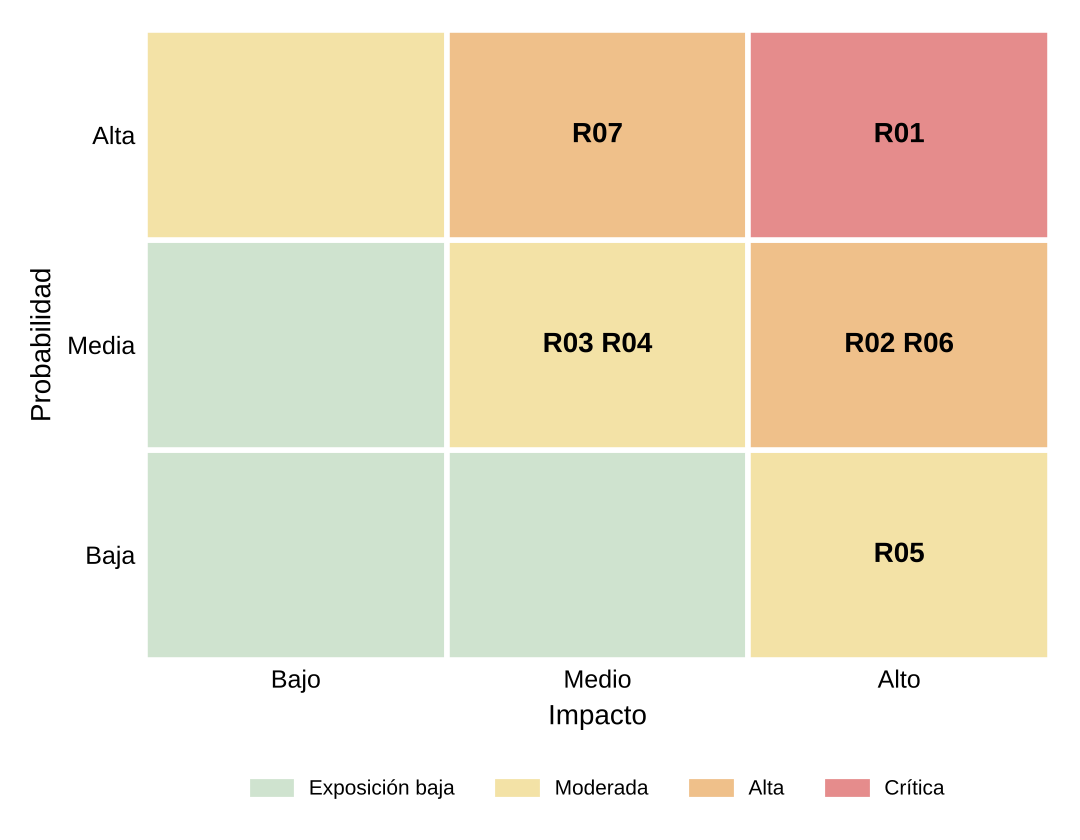
\includegraphics[width=0.75\textwidth]{matriz_exposicion_riesgos.png}
    \caption{Matriz de exposición de los riesgos R01--R07}
    \label{fig:matriz_exposicion_riesgos}
\end{figure}

La matriz detallada de identificación, análisis, mitigación, supervisión y contingencia se presenta a continuación en la Tabla \ref{tab:matriz_rmmm}.

{\scriptsize
\begin{xltabular}{\textwidth}{|>{\raggedright\arraybackslash}p{0.7cm}|>{\raggedright\arraybackslash}p{2.3cm}|>{\centering\arraybackslash}p{0.9cm}|>{\centering\arraybackslash}p{1.0cm}|X|X|X|>{\raggedright\arraybackslash}p{1.6cm}|}
    % --- Título y encabezado de la PRIMERA página ---
    \caption{Matriz de identificación, análisis y mitigación de riesgos enfocada en modelado}
    \label{tab:matriz_rmmm} \\
    \hline
    \textbf{ID} & \textbf{Descripción del riesgo} & \textbf{Prob.} & \textbf{Imp.} & \textbf{Mitigación} & \textbf{Supervisión} & \textbf{Contingencia} & \textbf{Resp.} \\
    \hline
    \endfirsthead

    % --- Encabezado que se repite en las páginas SIGUIENTES ---
    \multicolumn{8}{l}{\textit{Continuación de la Tabla \ref{tab:matriz_rmmm}}} \\
    \hline
    \textbf{ID} & \textbf{Descripción del riesgo} & \textbf{Prob.} & \textbf{Imp.} & \textbf{Mitigación} & \textbf{Supervisión} & \textbf{Contingencia} & \textbf{Resp.} \\
    \hline
    \endhead

    % --- Pie de tabla en páginas intermedias ---
    \multicolumn{8}{r}{\textit{Continúa en la siguiente página...}} \\
    \endfoot

    % --- Pie final de la tabla ---
    \endlastfoot

    % --- Contenido de las filas ---
    \textbf{R01} & Inconsistencia de nombres, atributos o métodos entre el diagrama de clases, los diagramas de secuencia y el modelo E-R. & Alta & Alto & Usar el glosario y el diccionario de datos como fuente única de nombres; realizar revisiones cruzadas lideradas por QA antes de cerrar cada iteración. & Lista de verificación de nomenclatura en cada auditoría; conteo de hallazgos por iteración (meta: cero críticos abiertos). & Congelar el diagrama afectado, tomar el diccionario de datos como referencia y corregir en una sesión conjunta de hasta un día. & QA \\*
    \hline
    \textbf{R02} & Ambigüedad en las reglas de negocio críticas (p. ej., descuento de \textit{stock} al confirmar el pedido o estados del pedido). & Media & Alto & Documentar precondiciones, postcondiciones y flujos alternativos en los casos de uso expandidos antes de elaborar las secuencias. & Revisión de los casos de uso expandidos por especialistas dinámicos y estructurales; registro de dudas abiertas en el acta de cada \textit{check-in}. & Adoptar provisionalmente la interpretación del Coordinador, documentarla como supuesto y revalidarla en la siguiente auditoría. & Coordinador y especialistas dinámicos \\*
    \hline
    \textbf{R03} & Desviación del alcance (\textit{scope creep}) al intentar programar prototipos funcionales en lugar de profundizar el modelado. & Media & Medio & Mantener el enfoque en los artefactos UML, el diseño de BD y los \textit{mockups} estáticos o navegables acordados en la Sección \ref{subsec:alcance_delimitacion}. & Contrastar en cada \textit{check-in} las tareas en curso con el cronograma y el alcance; vigilar la aparición de código en el repositorio. & Suspender la tarea fuera de alcance, retirarla de la rama principal y reasignar sus horas a artefactos pendientes. & Coordinador \\*
    \hline
    \textbf{R04} & Diferencias de notación UML o de estilo visual al dividir los diagramas entre los 7 integrantes. & Media & Medio & Estandarizar Draw.io como única herramienta, además de la paleta de colores y las convenciones de nomenclatura, desde la semana 1; publicar una plantilla base en el repositorio. & Revisión de notación y estilo en la auditoría de cada iteración. & Homogeneizar los diagramas con la plantilla; QA asigna la tarea a un integrante por iteración. & QA y arquitectura \\*
    \hline
    \textbf{R05} & Pérdida o desactualización de los archivos editables de diagramas o del documento. & Baja & Alto & Centralizar todos los archivos fuente (\texttt{.drawio}, \texttt{.tex} y exportaciones) en el repositorio GitHub, con \textit{commits} al cierre de cada sesión de trabajo. & QA verifica en cada \textit{check-in} que el último \textit{commit} refleje el avance reportado. & Restaurar la última versión desde el historial de Git o la copia local; reconstruir desde las exportaciones PNG/PDF si es necesario. & QA \\*
    \hline
    \textbf{R06} & Cambios o interpretaciones divergentes de los RF/RNF tras aprobarse la línea base de requerimientos (p. ej., lecturas distintas de RF11 y RF12). & Media & Alto & Congelar los requerimientos en LB-I1; tramitar todo cambio como solicitud de cambio; mantener actualizada la matriz de trazabilidad. & Comparar la matriz de trazabilidad con la versión vigente de los RF/RNF en cada auditoría; llevar el registro de solicitudes de cambio. & Evaluar el impacto con la matriz de trazabilidad, actualizar solo los artefactos afectados y generar una nueva versión con su acta. & Coordinador y QA \\*
    \hline
    \textbf{R07} & Conflictos de edición o sobrescritura de archivos de diagramas por el trabajo concurrente de varios integrantes. & Alta & Medio & Asignar un responsable único por artefacto; trabajar en ramas por artefacto y fusionar mediante \textit{pull request}; aplicar la convención de nombres de archivo. & Revisar en cada \textit{check-in} el historial de \textit{commits} y los conflictos de fusión reportados. & Resolver el conflicto desde el historial de Git conservando la versión de la línea base más reciente y reaplicar manualmente los cambios perdidos. & QA \\
    \hline
\end{xltabular}
}

\subsection{Mecanismos de Seguimiento y Control del Proyecto}
\label{subsec:seguimiento_control}

Para garantizar la calidad técnica de los modelos y el cumplimiento del cronograma de 3 semanas, el equipo aplica tres mecanismos de control complementarios: uno operativo (reuniones de sincronización), uno de verificación (auditoría de consistencia) y uno de cobertura (matriz de trazabilidad). Sus resultados alimentan la supervisión de la matriz RMMM y las métricas de la Sección \ref{subsec:esfuerzo_metricas}.

\subsubsection{Reuniones de sincronización cortas (\textit{check-ins})}
Sesiones breves de 15 minutos, realizadas cada dos días (aproximadamente diez en el ciclo de 3 semanas), conducidas por el Coordinador. Cada integrante informa qué avanzó, qué hará hasta la siguiente sesión y qué impedimentos tiene. Sirven para revisar el avance de cada diagrama, resolver dudas de lógica de negocio y evitar trabajo duplicado entre los 7 integrantes. Los acuerdos, los impedimentos y las dudas abiertas se registran en un acta breve almacenada en el repositorio; los impedimentos que persistan más de dos sesiones se escalan al Coordinador y se incorporan a la supervisión de riesgos.

\subsubsection{Auditoría de consistencia UML al cierre de cada iteración}
Revisión conjunta, liderada por el responsable de QA, en la que se verifica que cada clase, entidad y mensaje de los diagramas de secuencia coincida exactamente en nomenclatura y cardinalidad con el resto de los artefactos. Se aplica una lista de verificación que incluye: correspondencia entre clases, entidades y tablas; coincidencia de los mensajes de secuencia con métodos de clase; coherencia de los estados del pedido (\textit{Recibido}, \textit{En preparación}, \textit{En camino} y \textit{Entregado}) en los diagramas de actividades y de estados; y cumplimiento de la notación y de la plantilla visual. Los hallazgos se clasifican por severidad (crítico, mayor o menor) y se registran en el acta de auditoría con su responsable y su estado; no se cierra la línea base de la iteración mientras existan hallazgos críticos abiertos.

\subsubsection{Matriz de trazabilidad requerimiento-modelo}
Control cruzado que asegura que los 18 requerimientos funcionales (\texttt{RF01}--\texttt{RF18}) y los 11 no funcionales (\texttt{RNF01}--\texttt{RNF11}) estén debidamente representados en los artefactos de modelado. Cada RF debe vincularse al menos con un caso de uso, un elemento del modelo estructural o de datos, un diagrama dinámico y una pantalla del prototipo. Cada RNF debe vincularse al menos con un artefacto de diseño que lo atienda (arquitectura, modelo de datos o prototipo). QA crea la matriz en la Iteración 2, la actualiza al cierre de cada iteración y la utiliza para evaluar el impacto de las solicitudes de cambio; la cobertura esperada al cierre del proyecto es del $100\%$.

{\small
\begin{xltabular}{\textwidth}{|>{\raggedright\arraybackslash}p{3.4cm}|>{\raggedright\arraybackslash}p{3.0cm}|>{\raggedright\arraybackslash}p{2.4cm}|X|}
    % --- Título y encabezado de la PRIMERA página ---
    \caption{Resumen de los mecanismos de seguimiento y control}
    \label{tab:mecanismos_control} \\
    \hline
    \textbf{Mecanismo} & \textbf{Frecuencia} & \textbf{Responsable} & \textbf{Insumo} \\
    \hline
    \endfirsthead

    % --- Encabezado que se repite en las páginas SIGUIENTES ---
    \multicolumn{4}{l}{\textit{Continuación de la Tabla \ref{tab:mecanismos_control}}} \\
    \hline
    \textbf{Mecanismo} & \textbf{Frecuencia} & \textbf{Responsable} & \textbf{Insumo} \\
    \hline
    \endhead

    % --- Pie de tabla en páginas intermedias ---
    \multicolumn{4}{r}{\textit{Continúa en la siguiente página...}} \\
    \endfoot

    % --- Pie final de la tabla ---
    \endlastfoot

    % --- Contenido de las filas ---
    \textit{Check-ins} de sincronización & Cada 2 días (15 min) & Coordinador & Avance individual, impedimentos y dudas. \\*
    \hline
    Auditoría de consistencia UML & Al cierre de cada iteración (3) & QA & Diagramas, glosario, diccionario de datos y lista de verificación. \\*
    \hline
    Matriz de trazabilidad & Actualización al cierre de cada iteración & QA & RF/RNF vigentes y artefactos de cada iteración. \\
    \hline
\end{xltabular}
}

\subsection{Criterios de Aceptación y Definición de Terminado}
\label{subsec:criterios_aceptacion}

Los criterios de aceptación establecen las condiciones que debe cumplir cada entregable para ser admitido en una línea base, y la definición de terminado (DoD, \textit{Definition of Done}) fija las condiciones comunes que debe satisfacer cualquier artefacto, iteración y el proyecto en su conjunto.

\subsubsection{Criterios de aceptación por entregable}

{\footnotesize
\begin{xltabular}{\textwidth}{|>{\raggedright\arraybackslash}p{3.0cm}|X|>{\raggedright\arraybackslash}p{2.6cm}|}
    % --- Título y encabezado de la PRIMERA página ---
    \caption{Criterios de aceptación de los entregables}
    \label{tab:criterios_aceptacion} \\
    \hline
    \textbf{Entregable} & \textbf{Criterio de aceptación} & \textbf{Verifica} \\
    \hline
    \endfirsthead

    % --- Encabezado que se repite en las páginas SIGUIENTES ---
    \multicolumn{3}{l}{\textit{Continuación de la Tabla \ref{tab:criterios_aceptacion}}} \\
    \hline
    \textbf{Entregable} & \textbf{Criterio de aceptación} & \textbf{Verifica} \\
    \hline
    \endhead

    % --- Pie de tabla en páginas intermedias ---
    \multicolumn{3}{r}{\textit{Continúa en la siguiente página...}} \\
    \endfoot

    % --- Pie final de la tabla ---
    \endlastfoot

    % --- Contenido de las filas ---
    Requerimientos y glosario & 18 RF y 11 RNF identificados de forma única, redactados de manera verificable y sin contradicciones; glosario con los términos de negocio utilizados en los demás artefactos; alcance B2C sin pasarela de pagos ni rastreo GPS. & QA y Coordinador \\*
    \hline
    Casos de uso & Diagrama general con los actores Cliente y Administrador que cubre los 4 módulos; casos expandidos de los flujos críticos con actor, precondiciones, flujo principal, flujos alternativos y postcondiciones. & Especialistas dinámicos y QA \\*
    \hline
    Diagrama de clases & Clases, atributos, métodos y multiplicidades definidos; reglas de inventario y validación de disponibilidad (RF11) reflejadas; nombres coherentes con el glosario y el modelo E-R. & Especialistas estructurales y QA \\*
    \hline
    Modelo E-R, esquema relacional y diccionario de datos & Entidades, claves primarias y foráneas y cardinalidades definidas; esquema normalizado al menos hasta tercera forma normal; diccionario con tipo de dato MySQL, longitud, restricciones y descripción de cada atributo. & Especialistas estructurales y QA \\*
    \hline
    Diagramas de secuencia, actividades y estados & Cubren los flujos críticos de registro, catálogo, carrito, validación de \textit{stock}, confirmación y gestión de pedidos; los mensajes corresponden a métodos de clase; los estados del pedido (\textit{Recibido}, \textit{En preparación}, \textit{En camino} y \textit{Entregado}) tienen transiciones válidas. & Especialistas dinámicos y QA \\*
    \hline
    Diagramas de componentes y despliegue & Representan la arquitectura cliente-servidor web con sus capas de presentación, lógica y datos, y atienden al menos los RNF de seguridad, compatibilidad y mantenibilidad (RNF03, RNF06 y RNF09). & Arquitectura y QA \\*
    \hline
    Prototipos (\textit{wireframes} y \textit{mockups}) & Pantallas de Cliente y Administrador navegables, que cubren todas las funciones con interfaz de usuario de los RF, incluidos los mensajes de validación de disponibilidad; diseño adaptable a distintos tamaños de pantalla (RNF07) y estilo visual consistente. & UX/UI y QA \\*
    \hline
    Matriz de trazabilidad & Cobertura del $100\%$: cada RF vinculado a un caso de uso, un elemento estructural o de datos, un diagrama dinámico y una pantalla; cada RNF vinculado a un artefacto de diseño. & QA \\*
    \hline
    Informe final & Documento maestro integrado, con numeración y referencias de figuras y tablas, ortografía y puntuación revisadas y etiqueta \texttt{LB-I3} en el repositorio. & Coordinador y QA \\
    \hline
\end{xltabular}
}

\subsubsection{Definición de terminado de un artefacto}
Un artefacto se considera terminado cuando cumple todas las condiciones siguientes:
\begin{enumerate}
    \item Satisface los criterios de aceptación de su entregable (Tabla \ref{tab:criterios_aceptacion}).
    \item Emplea la notación UML, la nomenclatura y la plantilla visual estandarizadas por el equipo.
    \item Fue revisado por un integrante distinto de su autor y cuenta con el visto bueno de QA.
    \item No tiene hallazgos críticos ni mayores abiertos en la auditoría de consistencia.
    \item Su trazabilidad con los RF/RNF está registrada y actualizada en la matriz.
    \item Su fuente editable y su exportación (PNG / PDF) están en el repositorio, en versión 1.0 y fusionadas mediante \textit{pull request} aprobado.
    \item Está incluido en el documento maestro con leyenda, numeración y referencia en el texto.
\end{enumerate}

\subsubsection{Definición de terminado de una iteración y del proyecto}
\begin{itemize}
    \item \textbf{Iteración:} Todos los artefactos planificados cumplen la definición de terminado; la auditoría de consistencia se realizó y su acta está archivada; la matriz de trazabilidad y la matriz RMMM están actualizadas; y la etiqueta de línea base (\texttt{LB-I1}, \texttt{LB-I2} o \texttt{LB-I3}) fue creada.
    \item \textbf{Proyecto:} Las tres líneas base están cerradas; los 18 RF y los 11 RNF cuentan con cobertura del $100\%$ en la matriz de trazabilidad; el informe final fue entregado; y no se produjo ningún elemento de los excluidos en la Sección \ref{subsec:alcance_delimitacion}.
\end{itemize}